\chapter{Modelling a Digital Twin of 2 GW, 66 kV HVAC Offshore Network with MMC-HVDC Transmission}\label{4}
This chapter details the development of a multi-gigawatt (focus of 2 GW), 66 kV \gls{HVAC} offshore network connected to two offshore converter stations. Like in Chapter \ref{3}, an average \gls{EMT} modelling depth is used (i.e. focus on the study of three-phase faults occurring in a balanced system), the model is developed and simulations are conducted in RSCAD. The model depicts the connection of four \gls{OWF}s through a 66 kV \gls{HVAC} offshore network contributing a total of 2 GW installed capacity. The power is transferred to the onshore system through \gls{MMC} based \gls{HVDC} links. The focus is to investigate the dynamic performance of such a system when subjected to severe disturbances (e.g. three-phase line to ground fault) in the \gls{AC} part of the network. The role of both \gls{DVC} in \gls{WG}s and voltage control in \gls{MMC} is examined in detail to understand the voltage performance and the power flow distribution based on simulations performed in RSCAD. %Firstly, the topology selected for the network is explained, and then the large scale network layout with all the components is detailed. The control structures utilized in the network is described in the final part of this chapter.

\subsection{Processors in RSCAD}\label{split_system}
The simulations in RSCAD can be run in either NovaCor or PB5 processor cards. NovaCor processor is used for this work as they have 2-3 times the simulation capacity of a completely loaded PB5 processor \cite{noauthor_novacor_nodate_1}. For an extensive power system network, NovaCor processor requires a part of the system to be placed in a separate subsystem. RSCAD allows provision for splitting of the network into subsystems if the network is large. The splitting is done by right-clicking on the main subsystem tag and choosing "Add Subsystem" as shown in Figure \ref{fig:subsystem_RSCAD} and this feature is utilized in this section. Tline modules are used to connect subsystems. The process is explained in Section \ref{Tline_cable_RSCAD} in detail.

There are two NovaCor processors available at TU Delft and they are equipped with four cores each. These cores are utilized to solve the overall network solution, auxiliary components (such as transformers, cables, generators etc.) and the controls present in the simulation. Assignment of cores for solving various components of the network is an important step that needs to be considered while modelling, as they depict the total load that is distributed over the available cores. The process is detailed in Section \ref{Aggregated_OWF_large_scale}. 

\begin{figure}[H]
\centering
%\hspace*{-1.2cm}
    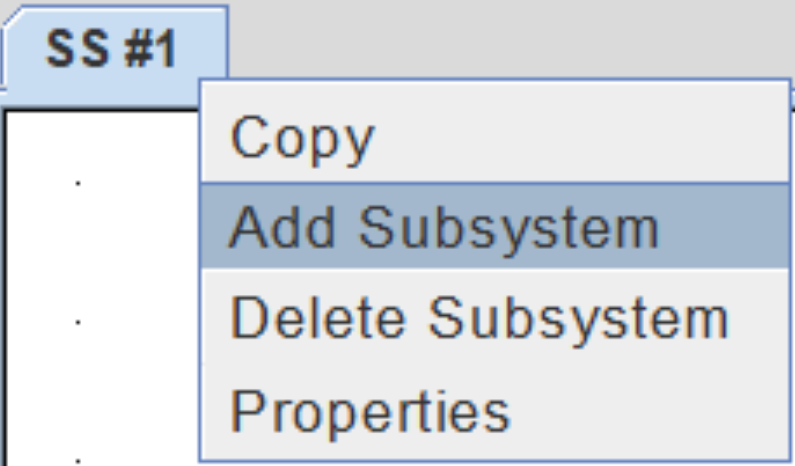
\includegraphics[height = 2cm,width = 3.5cm]{Diagrams/Chapter_3/Subsystem.PNG}
    \caption{Adding subsystems in RSCAD}
    \label{fig:subsystem_RSCAD}
\end{figure}


\section{Defining the layout for the 2 GW Offshore Network}
The initial aspect that needs to be considered for a offshore network is the topology of the network. The popularity of \gls{MMC} due to its improved controllability and superior system performances has led way for the increasing demand for \gls{MMC}-\gls{HVDC} transmission for integration of long distance \gls{OWF}s. For the connection of new \gls{OWF}s in the vicinity of the already existing ones, parallel operation of \gls{MMC}-\gls{HVDC} transmission systems can be expected in the near future with multiple connections to the onshore system. Such type of schemes increase the interest in hybrid systems with the hub-and-spoke principle proposed by ABB \cite{abb_hvdc_2018} and represented in Figure \ref{fig:ABB_Hub_Spoke_3}. The layout in Figure \ref{fig:ABB_Hub_Spoke_3}a) depicts the connection of \gls{OWF}s to a offshore converter station which in turn transfers power to the onshore system through multi-terminal \gls{HVDC} connections. However, in such a layout, the idea of scaling of offshore wind power is limited to the installed capacity of the \gls{MMC} unit. Another layout involves the \gls{OWF}s connected through \gls{AC} links to a back-to-back \gls{HVDC} converter station as shown in Figure \ref{fig:ABB_Hub_Spoke_3}b). Long distance \gls{HVAC} transmission is required in this case, for the transfer of power from \gls{OWF}s to the onshore network and hence contribute to high losses in the network when compared to \gls{HVDC} transmission for larger distances. Figure \ref{fig:ABB_Hub_Spoke_3}c) represents the connection of multiple \gls{OWF}s to the offshore converter station, and power is transferred to the onshore system through multiple \gls{HVDC} links. Such a layout provides contingency in the network by supplying offshore wind power to at least one onshore system if one of the \gls{HVDC} links gets disconnected \cite{lescale2012parallelling}. A stage-wise construction of such a \gls{HVDC} project is easier to be achieved by the developers as well \cite{cigre_B455}.

A specific configuration for a 2 GW offshore network is currently non-existent and this chapter tries to fill in such a research gap. The idea in this chapter is to expand the single \gls{OWF} model network in Figure \ref{fig:WT1_Model_RSCAD} for a 2 GW offshore wind power network. This could be made possible by connecting four such \gls{OWF} models in parallel with each generating 500 MW of power. The reason for choosing four \gls{OWF}s is to have a symmetrical layout and to test the ability of RSCAD to perform simulations of such a configuration. Correspondingly, a 2 GW offshore converter station capacity is required to transfer this generated amount of power to the onshore system. However, currently deployed (state-of-the-art) \gls{MMC}-\gls{HVDC} transmission, has a maximum rated capacity of 1.2 GW \cite{peralta2012detailed}. Hence, with the available technology, two \gls{MMC} offshore stations of 1 GW each will be required for 2 GW power transmission. Taking the aforementioned factors into account, a modified layout of Figure \ref{fig:ABB_Hub_Spoke_3}c) is developed for this work. 

\begin{figure}[H]
\centering
%\hspace*{-1.2cm}
    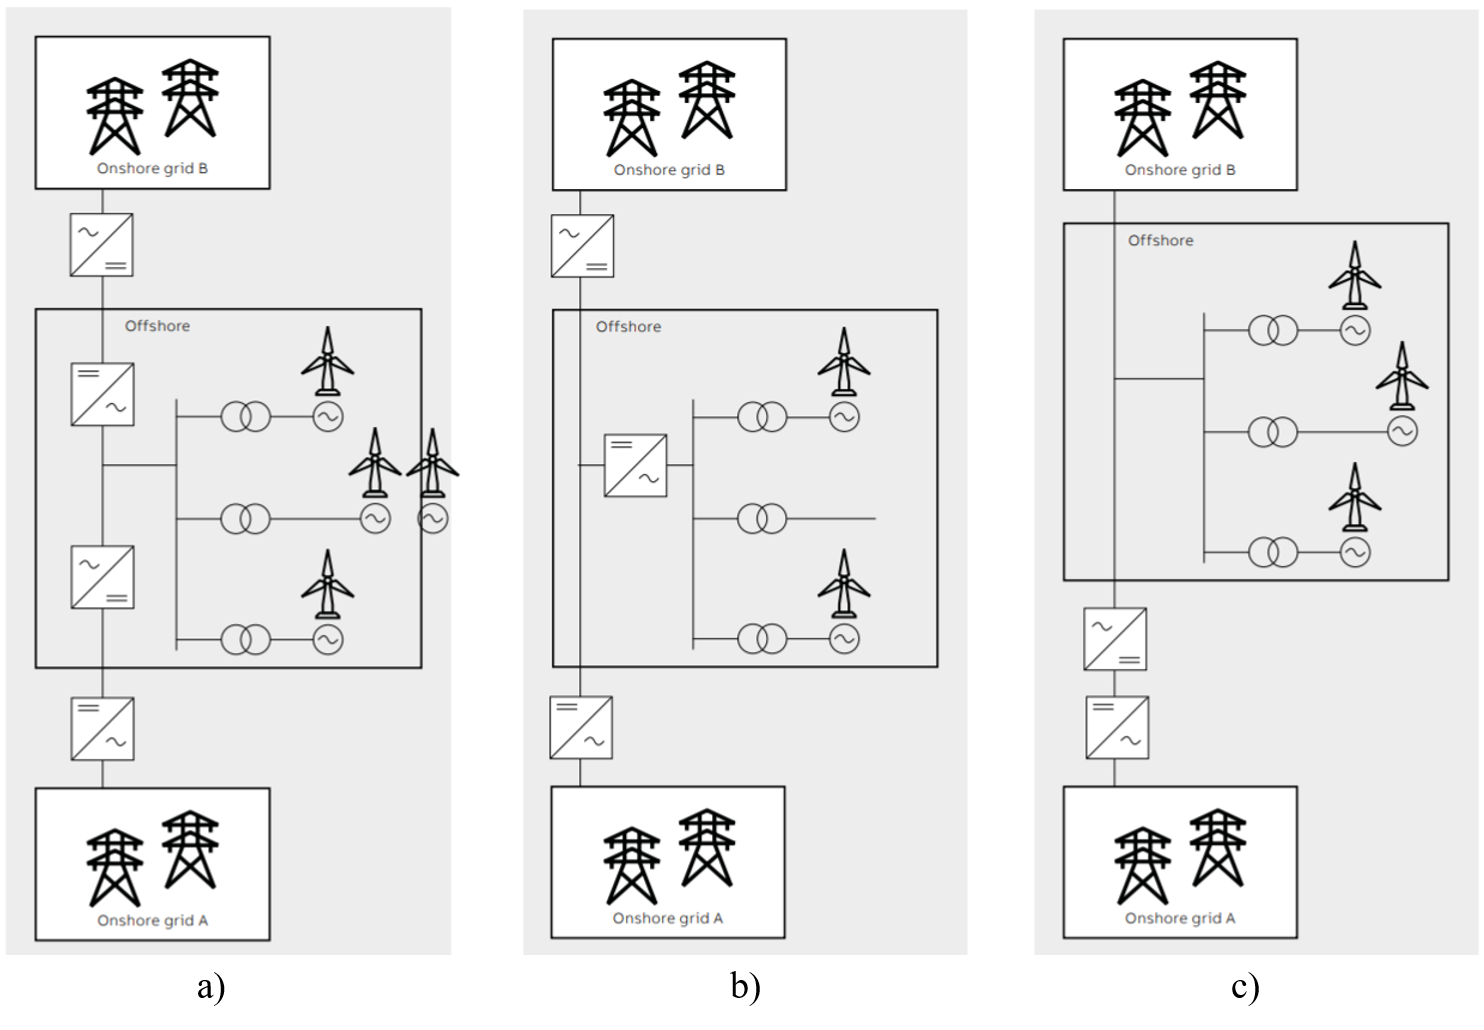
\includegraphics[height = 12cm,width = \textwidth]{Diagrams/Chapter_4/ABB_Hub_Spoke_3.png}
    \caption{a) Hub-and-spoke with multi-terminal HVDC system, b) Hub-and-spoke with AC links and HVDC back-to-back station and c) Hub-and-spoke with multiple HVDC links \cite{abb_hvdc_2018}}
    \label{fig:ABB_Hub_Spoke_3}
\end{figure}

\subsection{Scaling of single \gls{OWF} model for 2 GW offshore network}\label{scaling_2GW}

The layout of 2 GW network is built by resorting to scaling of the aggregated \gls{OWF} model in Section \ref{OWF} of Chapter \ref{3}. A modular topology is considered to achieve the capacity of 2 GW. 

\begin{itemize}
    \item The aggregated \gls{OWF} model in Section \ref{OWF} provides a generation of 700 MW. The first step involves reducing this generation to approximately 500 MW as the layout is planned for four \gls{OWF}s. This is achieved by reducing the number of parallel \gls{WG} units from 116 (116 x 6MW = 696 MW) to 83 (83 x 6MW = 498 MW) which is done by changing the scaling factor explained in Section \ref{scaling_OWF}. Now the \gls{OWF} generates nearly 500 MW of active power, as shown in Figure \ref{fig:Steps_for_Scaling}a).
    \item The second step involves connection of two \gls{OWF}s in parallel to the external \gls{AC} system in a modular approach. This allows for generation of 1 GW of power as depicted in Figure \ref{fig:Steps_for_Scaling}b). All the control structures incorporated in \gls{OWF}-1 are replicated for \gls{OWF}-2.
    \item In the third step, the external \gls{AC} system is replaced by an offshore converter station consisting of the average \gls{EMT} model of \gls{MMC} (\gls{MMC}-1) and the interface transformer (IT-1) available in the CIGRE B4 DC Grid Test System \cite{vrana2013cigre}. The same is depicted in Figure \ref{fig:Steps_for_Scaling}c). As the final layout network would be extensive it is required to split the network into subsystems, as mentioned in Section  \ref{split_system}. The splitting into two subsystems is performed in this step. The offshore converter station is modelled in subsystem-1 and the \gls{OWF}s are modelled in subsystem-2. \gls{MMC}-1 is designed to operate in V/F control (or grid forming control) which is explained at the end of this chapter.
    \item The final step involves parallel connection of two more \gls{OWF} models (\gls{OWF}-3 and \gls{OWF}-4) in a modular approach generating 500 MW each. Additionally, another offshore converter station consisting of a similar average \gls{EMT} model of \gls{MMC} (\gls{MMC}-2) and two interface transformers (IT-2a and IT-2b), is connected in parallel to the previous converter station. The need for two interface transformers in \gls{MMC}-2 bus is explained at the end of this chapter. Therefore, the final layout shown in Figure \ref{fig:WT4_MMC2} represents a total of 2 GW offshore wind power transmission.
\end{itemize}


% Therefore by using the average \gls{EMT} model of an \gls{MMC} described in utilizing the available models for \gls{MMC}s, to enhance and understand the operation of Type-4 \gls{WG}s in parallel operation and their coordination with \gls{MMC}s, an \gls{AC} collector grid topology with parallel connection of two point-to-point \gls{HVDC} transmission system is implemented for this thesis work in RSCAD. 



%The development of the layout involves major three steps:

%The layout of the model is developed by connecting four \gls{OWF} 


\begin{figure}[H]
%\centering
%\hspace*{-1.2cm}
    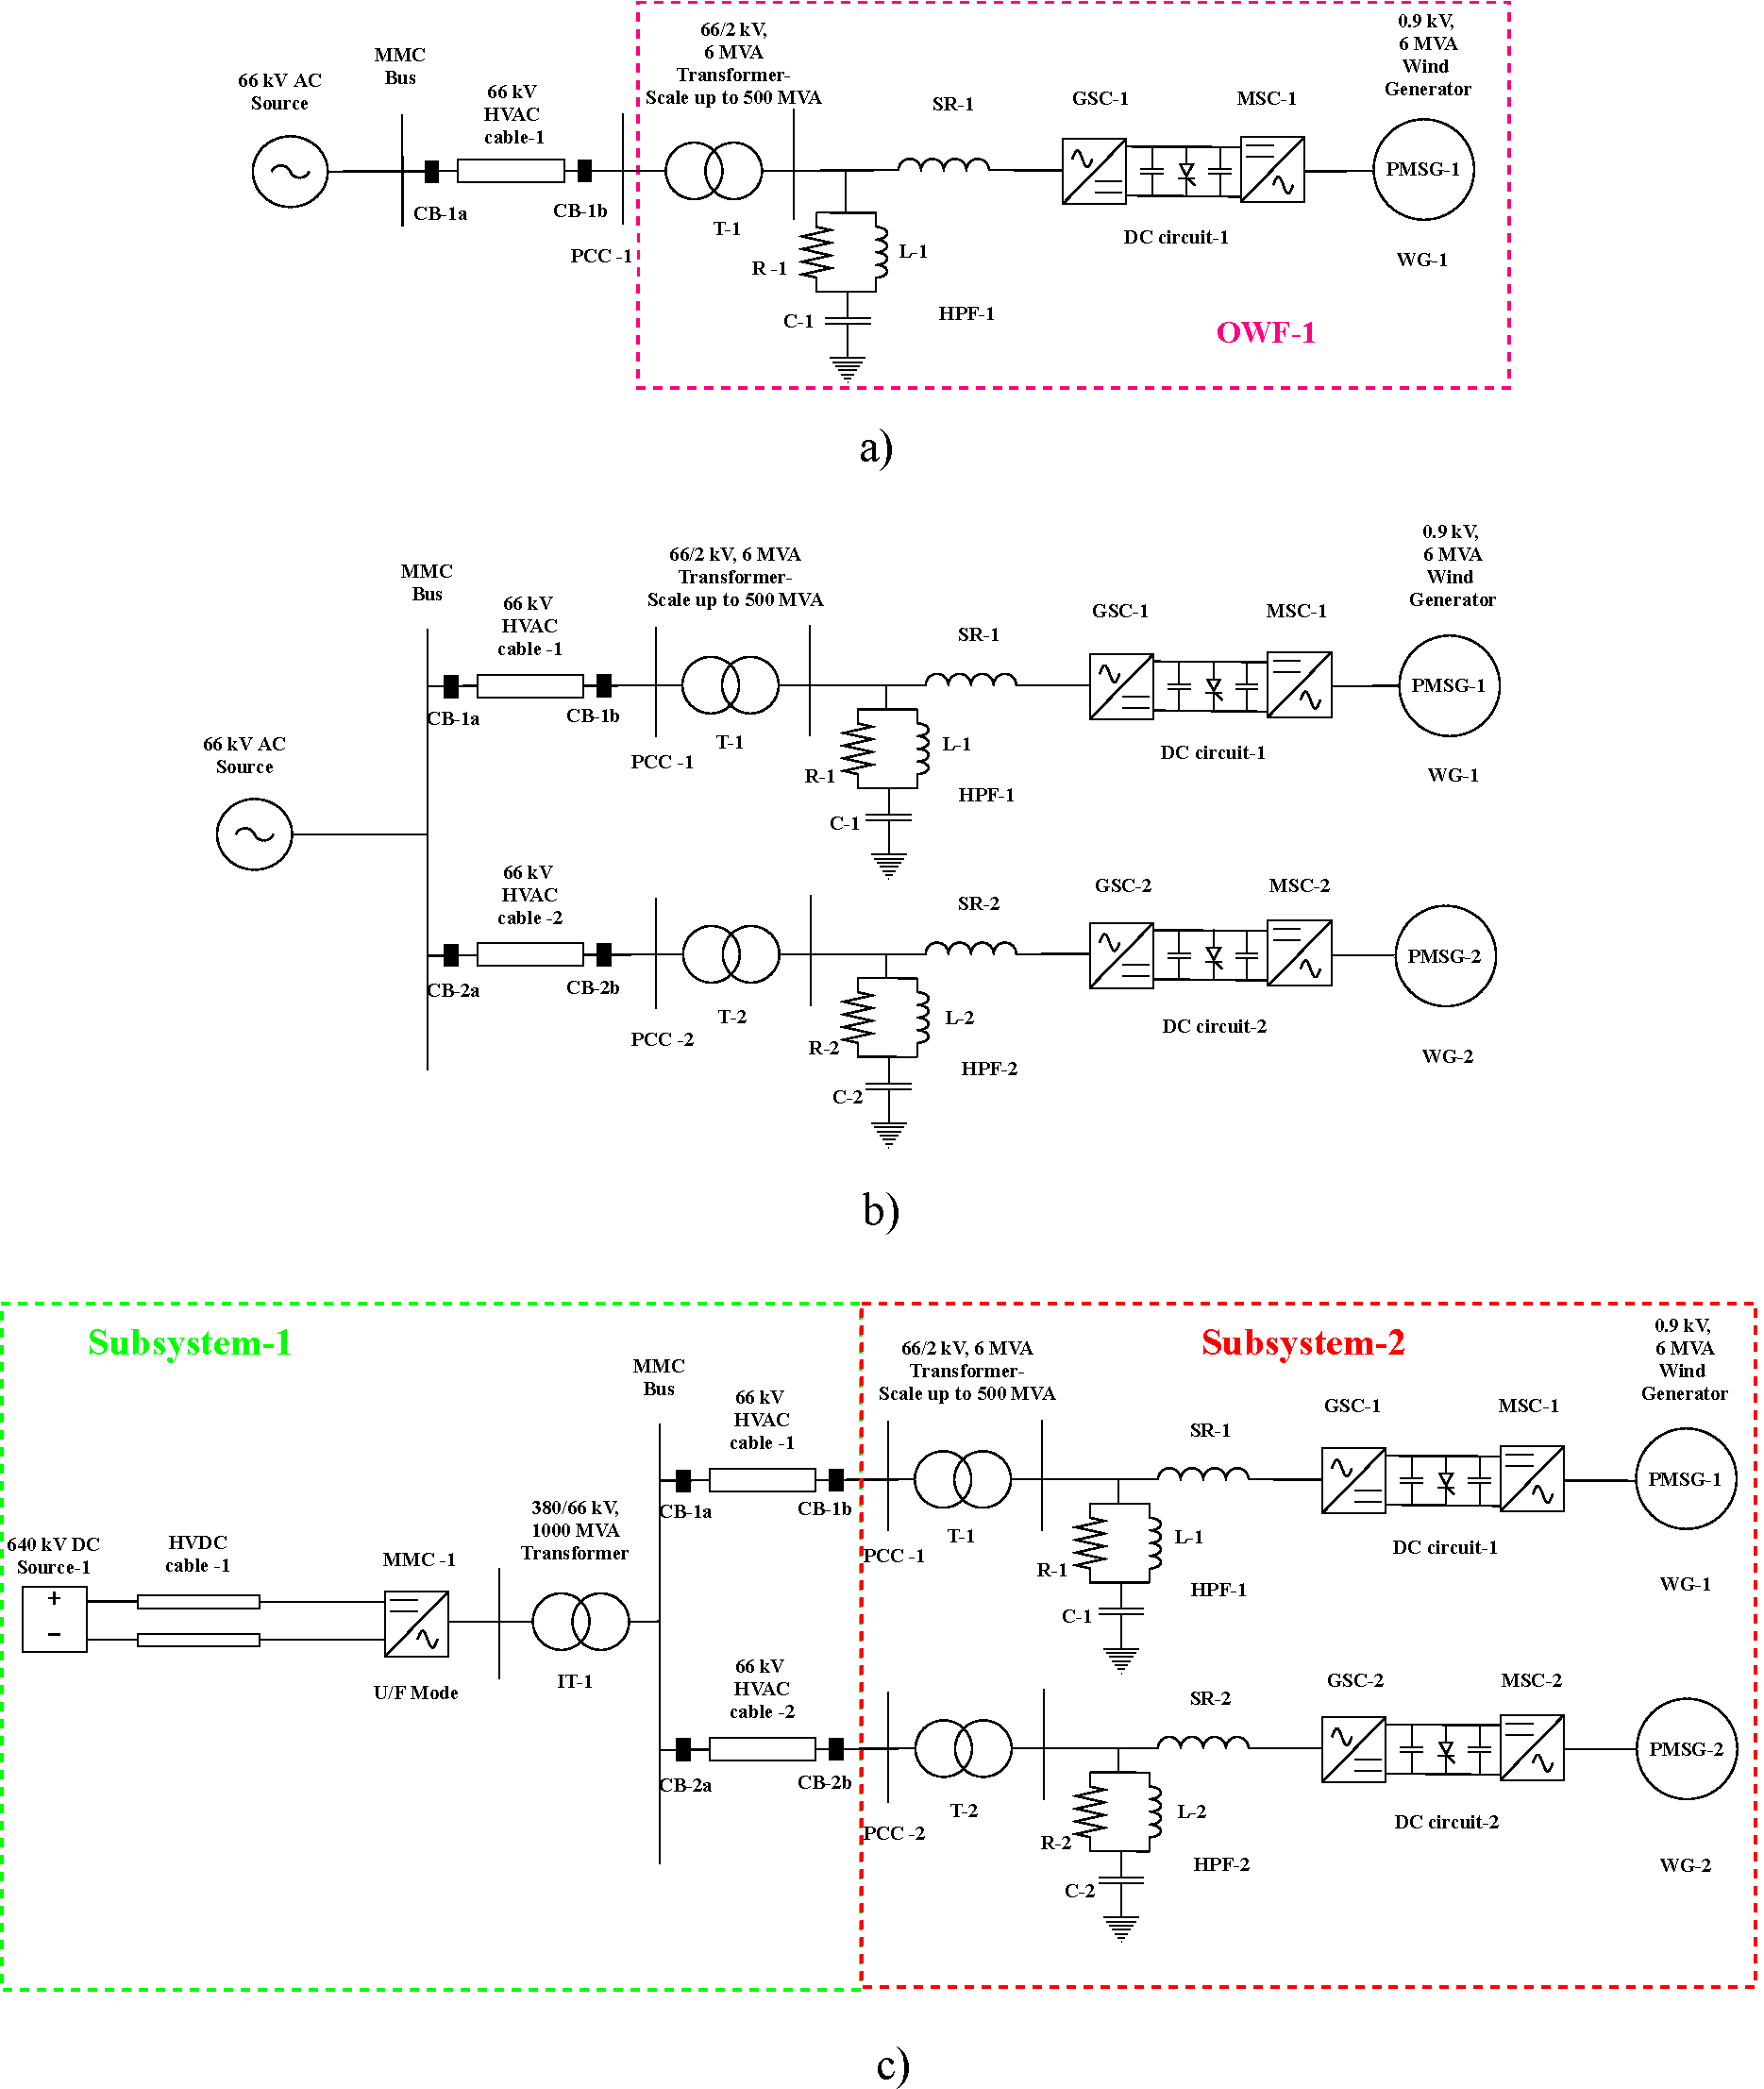
\includegraphics[height = 21cm,width = \textwidth]{Diagrams/Chapter_4/Steps_for_Scaling.pdf}
    \caption{a) OWF-1 connected to external AC system, b) OWF-1 and OWF-2 connected in parallel to external AC system c) OWF-1 and OWF-2 connected in parallel to MMC-1}
    \label{fig:Steps_for_Scaling}
\end{figure}

\begin{figure}[H]
%\centering
%\hspace*{-1.5cm}
    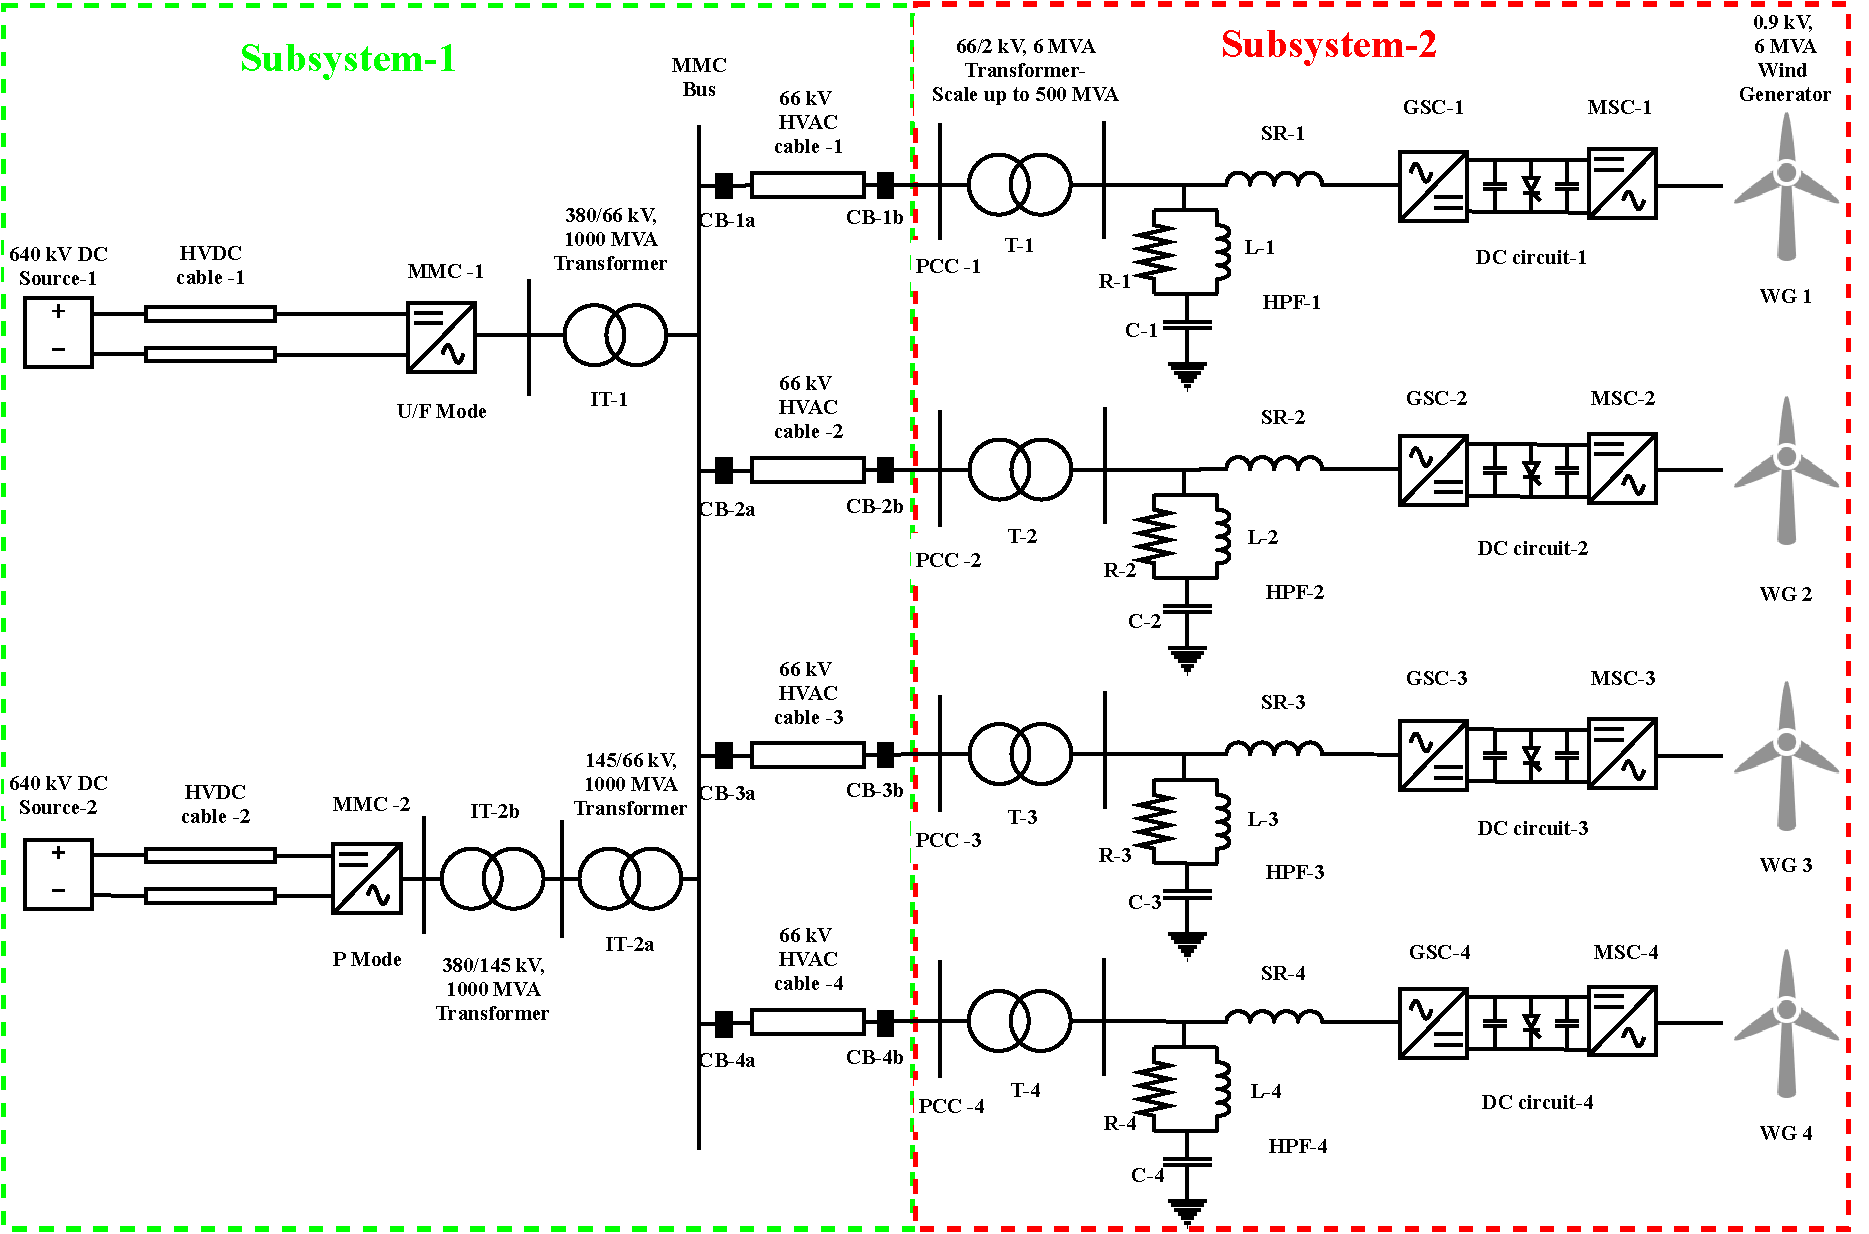
\includegraphics[height = 12cm,width = \textwidth]{Diagrams/Chapter_4/WT4_MMC2_new.pdf}
    \caption{Single line diagram of 2 GW, 66 kV HVAC offshore network connected to 2 x 1 GW HVDC links with offshore converter stations in RSCAD}
    \label{fig:WT4_MMC2}
\end{figure}

\section{Layout of 2 GW, 66 kV HVAC Offshore Network in RSCAD}

The components in the 2 GW, 66 kV \gls{HVAC} network is detailed in this section. The single line diagram of the network is depicted in Figure \ref{fig:WT4_MMC2} and the major components of the network include :
\begin{itemize}
    \item Four aggregated \gls{OWF}s, each with 500 MW installed capacity represented by the following components:
    \begin{itemize}
        \item A single Wind Generation System with 
    \begin{itemize}
        \item Permanent Magnet Synchronous Generator (\gls{PMSG})
        \item Machine Side Converter (\gls{MSC})
        \item \gls{DC} circuit
        \item Grid Side Converter (\gls{GSC}) 
    \end{itemize}
        \item High Pass filter (\gls{HPF}) with series reactor
        \item \gls{OWF} transformer
    \end{itemize}
    \item Four \gls{HVAC} cables  
    \item Three interface transformers
    \item Two \gls{MMC}s
    \item Two pairs of \gls{HVDC} cables
\end{itemize}

\subsection{Aggregated OWF}\label{Aggregated_OWF_large_scale}
As mentioned in Section \ref{scaling_2GW}, the 2 GW offshore wind power is split into four \gls{OWF}s with 500 MW rated capacity each. Currently, the largest offshore \gls{WG} developed by GE Renewable Energy has a rating of 12 MW \cite{noauthor_worlds_2020}. However, the standard model available for a Type-4 \gls{WG} in RSCAD is rated 6 MW. Hence, to represent a 500 MW \gls{OWF}, 83 \gls{WG}s are required. All the \gls{OWF}s are at a distance of 30 kms from the \gls{MMC} bus. 


The average model of Type-4 \gls{WG} available in RSCAD is used for this work as well. The aggregated \gls{OWF} model represented in small time step environment described in Section \ref{OWF} is used here for all the four \gls{OWF}s. As the entire network is extensive, it is split into two subsystems in RSCAD as shown in Figure \ref{fig:WT4_MMC2} by employing the technique explained in Section \ref{split_system}. The four \gls{OWF}s are modelled in subsystem-2 and the rest of the system is modelled in subsystem-1. Each subsystem requires one rack for operation and hence two NovaCor racks are used for the network simulation. It is also possible to simulate the network with PB5 processor. However, this requires a total of three subsystems since PB5 racks allow only small network solutions to be solved in one rack \cite{noauthor_pb5_nodate_1}. Therefore, two \gls{OWF}s are to be modelled in subsystem-3, other two \gls{OWF}s in subsystem-2 and the rest of the network in subsystem-1. Henceforth, the simulations are considered only in NovaCor processor for this study.  


Since there need to be four different small time step blocks representing four \gls{OWF}s, each block needs to be set with different step sizes so as to avoid conflict during initialization. These step sizes are only used for initialization and the actual step sizes can be viewed in the "Map File" as mentioned in Section \ref{OWF}. Moreover, if the time steps are not initialized properly, it could lead to the occurrence of a time step overflow error during the simulation in the Runtime module. 


Another important parameter to be considered here is the assignment of the cores for the small time step blocks. As mentioned in Section \ref{split_system}, cores are responsible for solving the entire network solution. NovaCor processor in TU Delft is configured with four cores and each component used in the network can be assigned to specific cores (1 to 4 in number). Since there are six small time step blocks (\gls{OWF}-1, 2, 3 and 4; \gls{MMC}-1 and \gls{MMC}-2) in total, the cores need to be manually assigned to each block to allocate the load on each processor within their capacity. The core allocation of the small time step blocks representing \gls{OWF}s for this network is chosen as shown in Table \ref{tab:Core_assignment_sub2}.  

   

\begin{table}[H]
\centering
\begin{tabular}{|c|c|}
\hline
\textbf{Small time step block} & \textbf{Core assignment} \\ \hline
OWF-1                          & 4                        \\ \hline
OWF-2                          & 1                        \\ \hline
OWF-3                          & 3                        \\ \hline
OWF-4                          & 1                        \\ \hline
\end{tabular}
\caption{Core assignment of OWF models in subsystem-2}
\label{tab:Core_assignment_sub2}
\end{table}

\subsection{HVAC Cables}\label{Tline_cable_RSCAD}
The \gls{HVAC} cables transfer power from the \gls{OWF}s to the offshore converter stations. Hence, four sets of \gls{HVAC} cables are required to transfer power from four \gls{OWF}s. The cables are rated at 66 kV and are 30 kms of length. In the network layout represented in RSCAD, as shown in Figure \ref{fig:WT4_MMC2}, the \gls{HVAC} cables connect the \gls{OWF}s in subsystem-1 with the \gls{MMC} bus in subsystem-2. To provide such a connection between components placed in different subsystems in RSCAD, a feature called Tline module is available in the RSCAD modules section (denoted by a red box in Figure \ref{fig:TlineModule_mark}). This module is similar to the Cable module explained in Section \ref{HVAC_cable_RSCAD}. However, Cable module only allows connection between components in the same subsystem. The Tline module can be modelled as overhead transmission line or cable. Since an offshore network model is considered in this work, the Tline model represents a subsea cable model. 

The cables are modelled as Bergeron models with RLC data parameters. Bergeron model is chosen to test the working of the network using travelling wave model. Moreover, as the 2 GW offshore network is developed from the single \gls{OWF} model in Section \ref{OWF}, the same RLC cable parameters used in Section \ref{HVAC_cable_RSCAD} are used in the Tline module for all the four sets of cables. 
 
 \begin{figure}[H]
\centering
%\hspace*{-1.2cm}
    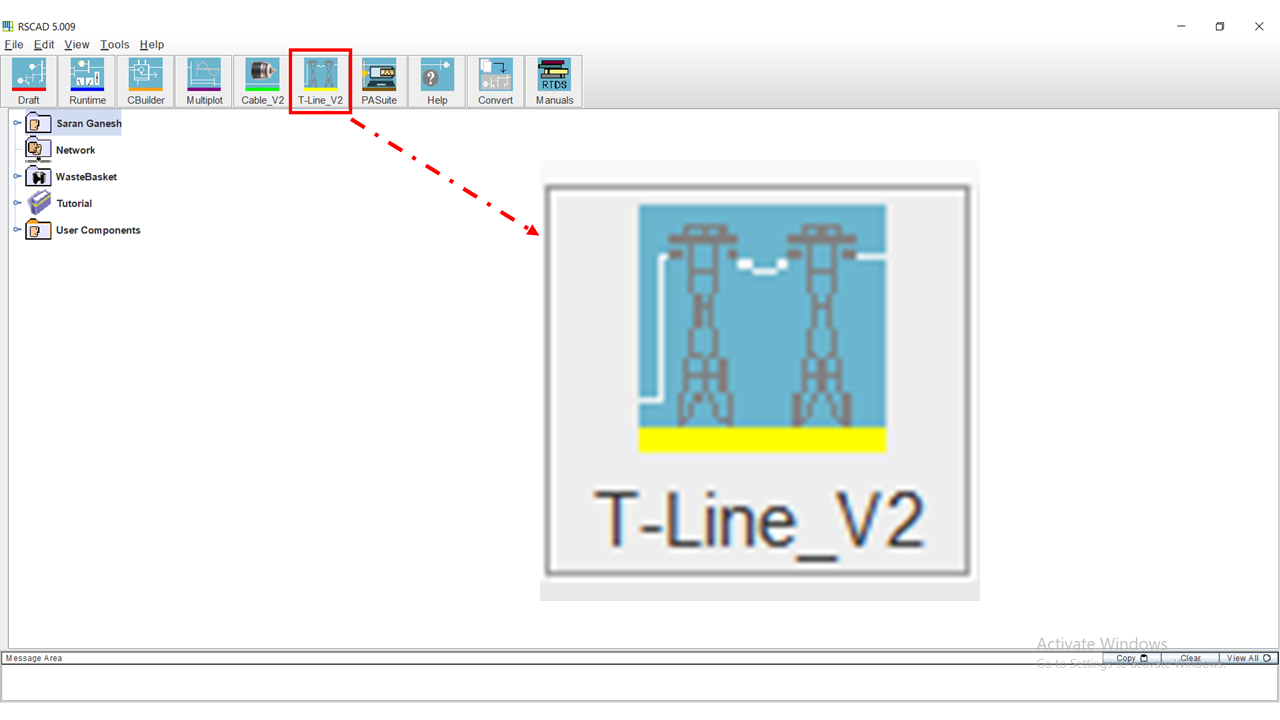
\includegraphics[height = 4.5cm,width = 7.5cm]{Diagrams/Chapter_4/Tline_module_Final.png}
    \caption{Tline module in RSCAD}
    \label{fig:TlineModule_mark}
\end{figure}
 
 In the Draft module, the cable model is added in the circuit using the unified Tline model shown in Figure \ref{fig:Tline_calculationbox_RSCAD} available in RSCAD power system library. The unified model consists of the following components: 
%\setlist{nolistsep}
    \begin{itemize}[noitemsep]
    \item Calculation Block
    \item Sending End Terminal
    \item Receiving End Terminal
\end{itemize}

The detailed representation of the cable parameters in Tline module, and the representation of the cable model using the calculation block, sending end terminal and receiving end terminals in the Draft module is shown in Appendix \ref{config_Tline}.

\begin{figure}[H]
  \centering
  % include first image
  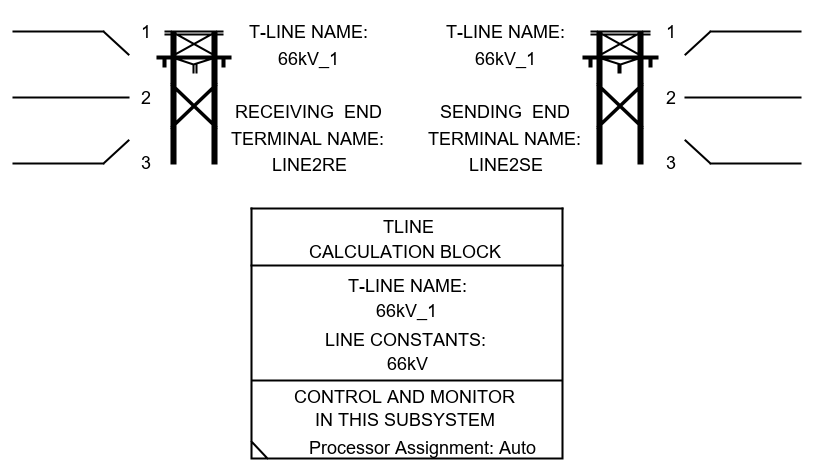
\includegraphics[height = 5cm,width = 8cm]{Diagrams/Chapter_4/TlineParaBlock.PNG}  
  \caption{Tline configuration in Draft module in RSCAD}
  \label{fig:Tline_calculationbox_RSCAD}
\end{figure}

As the significant goal is to estimate the dynamic performance of the network under severe disturbances, a three-phase short circuit event in the middle of \gls{HVAC} cable-1 is chosen. To perform a short circuit event in the middle of a 30 km long \gls{HVAC} cable in RSCAD, two cable models of 15 kms length are modelled and connected in series, and the three-phase fault logic available in RSCAD library is modelled in the middle of the two cables as shown in Figure \ref{fig:Subsystem_Trial}. It must be noted that each cable model contain one set of sending and receiving end terminals. In order to connect two subsystems, the sending end terminal from the \gls{OWF} is placed in subsystem-2, and its receiving end is placed in subsystem-1. %The representation of one \gls{OWF} and one set of \gls{HVAC} cable in two subsystems in RSCAD is shown in Figure  \ref{fig:Subsystem_Trial}. All \gls{OWF}s placed in subsystem 2 are connected to the rest of the system in system 1 using \gls{HVAC} cables in a similar fashion.

\begin{figure}[H]
\centering
%\hspace*{-0.8cm}
    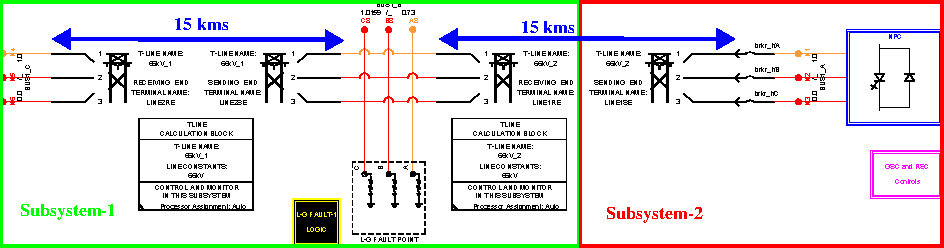
\includegraphics[height = 5.4cm,width = 17cm]{Diagrams/Chapter_4/subsystem_fault_mark.pdf}
    \caption{Representation of three-phase line to ground fault in the middle of HVAC cable-1 in RSCAD}
    \label{fig:Subsystem_Trial}
\end{figure}

\section{Offshore Converter Stations}
The offshore converter stations convert the \gls{HVAC} offshore wind power to \gls{HVDC} to transfer the power to the onshore system through \gls{HVDC} links.  %There are two offshore \gls{MMC} stations utilized in this network. 
The existing available \gls{HVDC} links in the industry have a rated capacity of 1.4 GW. Examples for such projects are the NordLink cable connecting Norway and Denmark, NSN Link connecting Norway and the United Kingdom \cite{ryndzionek_evolution_2020}. Moreover, the standard \gls{EMT} models for \gls{MMC}s available in CIGRE B4 DC Grid Test System \cite{vrana2013cigre} have a rated capacity of 1.2 GW. Therefore, with the currently available technology, two offshore converter stations are required for the transfer of 2 GW offshore wind power. From the description of \gls{MMC} explained in Section \ref{HVDC_trans_theory}, it can be understood that \gls{MMC}s also involve \gls{PE} components. Hence, similar to the \gls{OWF} model, the average \gls{EMT} models of \gls{MMC}s are represented in the small time step blocks in RSCAD to accurately represent fast switching events. The average \gls{EMT} models available in RSCAD consists of the \gls{MMC} and interface transformer modelled in the small time step environment representing the offshore converter station. For this work, two small time step blocks are required for the representation of two offshore converter stations. Both the blocks are placed in subsystem-1. These two blocks must be initialized with different time step to avoid conflict during initialization, and thereby avoiding the time step overflow error during the start of simulation in the Runtime module. To evenly distribute the load on four cores, considering the core allocation for \gls{OWF}s in Table \ref{tab:Core_assignment_sub2}, the cores for \gls{MMC}s are allocated as shown in Table \ref{tab:Core_assignment_sub1}. The offshore converter station-1 consists of the interface transformer (IT-1) and \gls{MMC}-1 whereas offshore converter station-2 consists of the interface transformers (IT-2a, IT-2b) and \gls{MMC}-2. 
%RSCAD also allows modelling in substep environment that can have a time step as small as 500 ns if the circuit is simple.    

\begin{table}[H]
\centering
\begin{tabular}{|c|c|}
\hline
\textbf{Small time step block} & \textbf{Core assignment} \\ \hline
MMC-1                          & 3                        \\ \hline
MMC-2                          & 2                        \\ \hline

\end{tabular}
\caption{Core assignment of MMC models in subsystem-1}
\label{tab:Core_assignment_sub1}
\end{table}


\subsection{Interface Transformers}
The interface transformers (also termed as converter transformers) are connected to the \gls{AC} side of the \gls{MMC}s and are depicted as IT-1 for offshore converter station-1 and IT-2a and IT-2b for offshore converter station-2 as shown in Figure \ref{fig:WT4_MMC2}. As explained in \cite{cigre2005b4}, these transformers entail the following main implications:
\begin{itemize}
    \item Providing a reactance between the offshore grid and the \gls{MMC}.
    \item Preventing the flow of zero sequence currents between the offshore grid and the \gls{MMC}.
\end{itemize} 

 %The three-phase three identical single-phase transformer \gls{VSC} interface model available in the RSCAD library shown in Figure \ref{fig:InterfaceTrafo} is considered for this research. 
As mentioned in the previous section, in the available average \gls{EMT} models in RSCAD library, the interface transformer is modelled with the \gls{MMC} in a small time step environment in RSCAD. Considering a delta-star type interface transformer and connecting \gls{MMC} to the delta side of the transformer, allows for isolation of the zero sequence currents during faults. The available \gls{EMT} models for offshore \gls{MMC} stations from \cite{vrana2013cigre} are utilized for this work. These models are designed for 145 kV \gls{HVAC} offshore network. Hence, to utilize this model for this work, the secondary side voltage of the transformer is changed from 145 kV to 66 kV. Additionally, there were modifications required to be made in the control structures of the \gls{MMC} models to utilize it for the 66 kV \gls{HVAC} network. These are explained in further sections of this chapter. There are mainly three interface transformers used in this work. The transformer (IT-1) is rated 66/380 kV, 1000 MVA in the offshore converter station-1. Two interface transformers in the offshore converter station-2 are rated 66/145 kV, 1000 MVA (IT-2a) and 145/380 kV, 1000 MVA (IT-2b) respectively. The need for two interface transformers in offshore converter station-2 is explained in the last section of this chapter.
%Due to limitation of the control structure model in RSCAD, an additional transformer is required to convert from 66 kV to 145 kV in the \gls{MMC}-2 bus. To have a minimum effect on the impedance of the network, the leakage inductance value of this transformer is kept as low as possible. In a practical scenario, this can be avoided by using a 66/380 kV transformer directly. 

\begin{comment}
\begin{figure}[H]
\centering
%\hspace*{-1.2cm}
    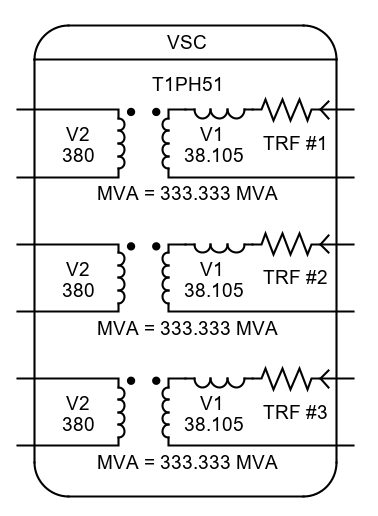
\includegraphics[height = 5cm,width = 4cm]{Diagrams/Chapter_4/InterfaceTrafo.PNG}
    \caption{VSC interface transformer model in RSCAD}
    \label{fig:InterfaceTrafo}
\end{figure}


These available models are for 145kV \gls{AC} offshore network. Since 66 kV \gls{HVAC} network is utilized for this work, the voltage rating on the secondary side of the transformer is changed to 66 kV. As the available models for the offshore \gls{MMC} station with the control structures are designed for 145 kV offshore network, a work around to use these models to be suitable for the 66 kV network is achieved.
\end{comment}

\subsection{Modular Multilevel Converters (MMCs)}
As mentioned in Chapter \ref{1}, it is seen that Modular Multilevel Converters (\gls{MMC}) are the present converter topology preferred for \gls{VSC}-\gls{HVDC} transmission schemes due to their high efficiency and other advantages. They prove to be the state-of-the-art technology for \gls{HVDC} transmission until today. The average \gls{EMT} model of \gls{MMC} in
RSCAD has the option of modelling the \gls{MMC} using half-bridge submodules or full-bridge submodules \cite{noauthor_mmc_nodate_1}. 
% The voltage level determines the number of submodules required. The highest levels for \gls{HVDC} projects range from 525 kV to 600 kV. The voltages are bound to increase for the bulk transfer of power in the future projects \cite{alassi2019hvdc}.
The voltage levels for \gls{HVDC} offshore wind farm projects in Europe range from 300 kV to 640 kV \gls{DC} voltage \cite{ryndzionek_evolution_2020}. Hence, to continue with the latest trend, voltage level of 640 kV \gls{DC} is chosen for this work. Therefore, 320 submodules are required per arm to create a voltage of $\pm$ 320 kV for the positive and negative poles. Both the \gls{MMC}s (\gls{MMC}-1 and \gls{MMC}-2) in the offshore converter stations are modelled for 640 kV \gls{DC}.  

\begin{comment}
Both the \gls{MMC}s are connected to the \gls{DC} sources through a symmetric monopole configuration with $\pm$ 320 kV rated voltage on the \gls{DC} side and 380 kV on the \gls{AC} side. 
 A Bergeron travelling wave transmission model is used to connect the \gls{MMC} in the small-time step network with the large time step network. The \gls{MMC} models considered for this research are modelled from the reference models in \cite{wachal2014guide}. \gls{DC} side of \gls{MMC}s are simplified by connecting the \gls{HVDC} cables to \gls{DC} sources since the area of study for this thesis is the \gls{AC} offshore network. 


\begin{figure}[H]
\centering
%\hspace*{-1.2cm}
    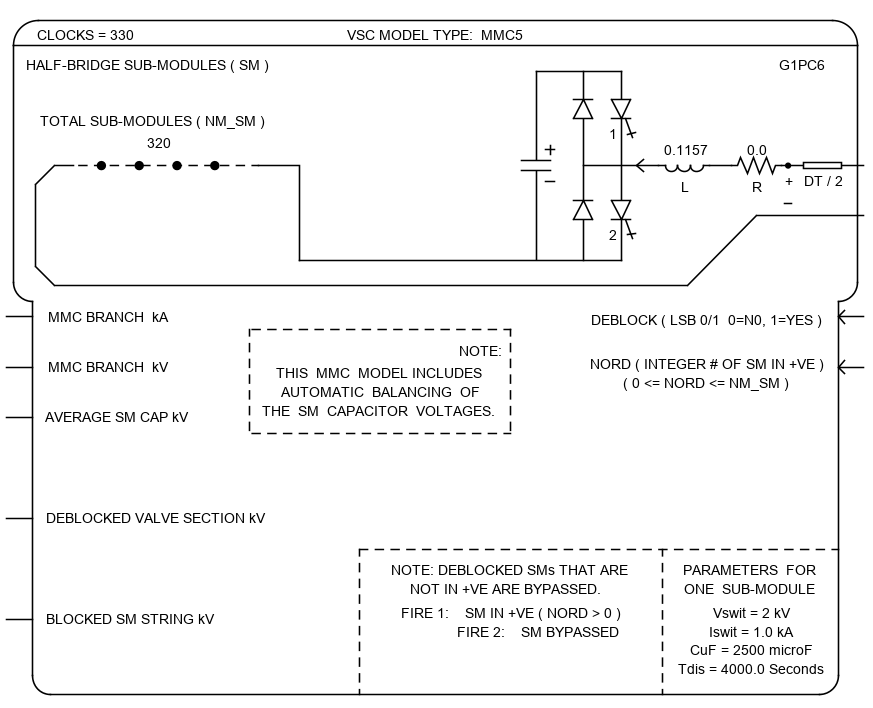
\includegraphics[height = 7cm,width = 9cm]{Diagrams/Chapter_4/MMC5_RSCAD_2.PNG}
    \caption{MMC model in RSCAD}
    \label{fig:MMC5_RSCAD_2}
\end{figure}
\end{comment}

\section{\gls{HVDC} Cables}
The \gls{HVDC} cables transfer the generated wind power from the offshore converter station to the onshore system. As mentioned in the above section, the voltage level chosen for \gls{HVDC} transmission in this work is 640 kV \gls{DC}. Therefore, each cable model must be suitable for $\pm$ 320 kV. The cable parameters available in \cite{vrana2013cigre} for $\pm$ 400 kV voltage are utilized in this work. The cable model is represented in frequency-dependent phase domain using the unified cable model block as explained previously in Section \ref{HVAC_cable_RSCAD} \cite{rtds_tech}. The cables are modelled in subsystem-1 and are labelled as \gls{HVDC} cable-1 and \gls{HVDC} cable-2 for the connection from offshore converter station-1 and offshore converter station-2 to the onshore system  respectively (Figure \ref{fig:WT4_MMC2}). 

\section{Onshore Equivalent Converter Stations}
The connection between the offshore converter station and the onshore converter station follows a symmetrical monopole configuration as shown in Figure \ref{Monopole_rep} \cite{sharifabadi2016design}. However, the \gls{DC} part of the onshore converter stations are represented using an equivalent \gls{DC} source for this work as shown in Figure \ref{Monopole_rep_2}. This is done, as the focus of the thesis is majorly on the dynamic performance related to the \gls{AC} side of the network. Conventionally, the onshore converter stations provide \gls{DC} voltage and reactive power control. Hence, the representation of a constant \gls{DC} voltage source ensures the \gls{DC} voltage control during the time of disturbances in the \gls{AC} offshore network. The voltage of the \gls{DC} sources are rated at 640 kV representing the \gls{HVDC} transmission voltage.  

\begin{figure}[H]
\centering

\subfloat[Symmetrical monopole configuration \cite{sharifabadi2016design}]{%
  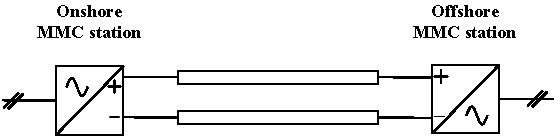
\includegraphics[clip,width=0.65\columnwidth]{Diagrams/Chapter_4/Monopole_rep.pdf}%
\label{Monopole_rep}}


\subfloat[Symmetrical monopole configuration by equivalent representation of DC side of onshore MMC station using a constant DC source]{%
  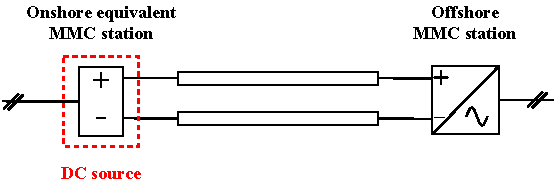
\includegraphics[clip,width=0.65\columnwidth]{Diagrams/Chapter_4/Monopole_rep_2.pdf}%
\label{Monopole_rep_2}}


\caption{Symmetrical monopole configuration in HVDC network}

\end{figure}



\section{Control structures}\label{control_structures}
This section explains the different control structures implemented and modifications required in the control scheme of converters for operation in the 66 kV \gls{HVAC} network. The \gls{DVC} inspired from \cite{erlich_new_2017} and implemented in Section \ref{DVC_RSCAD} for Type-4 \gls{WG}s is extended for the 2 GW network. There are mainly three control strategies used:
\begin{itemize}
    \item \gls{DVC} in the \gls{GSC}s of the \gls{WG}s used to represent aggregated \gls{OWF}s 
    \item Island mode control in \gls{MMC}-1
    \item Non- island mode control in \gls{MMC}-2
\end{itemize}

\subsection{DVC}
The control structure explained in Section \ref{DVC_RSCAD} is implemented for all the four \gls{WG}s. Since the same type of model is used for \gls{GSC}s in all four \gls{WG}s, the control loop parameters remain the same. The reactive and active control loop parameters are provided in Appendix \ref{tab:Reactive_pow_para} and \ref{tab:Active_pow_para} respectively.

\subsection{Island mode control}
It is highly necessary to use a control strategy in any of the \gls{MMC}s which could provide the voltage and frequency reference for the \gls{MMC} bus since it is connected to a weak network (\gls{OWF} network). The reference voltage is created by V/F control mode, which comes under the classification of islanded mode of control for \gls{VSC} \cite{vrana2013cigre}. For this study, \gls{MMC}-1 is operated in the V/F control. A basic control strategy was developed according to the illustration provided in \cite{wachal2014guide} and is shown in Figure \ref{fig:U_F_control}. Since the voltage angle reference ($\theta$), is generated by an independent Voltage Controlled Oscillator (VCO), this control is termed under island mode operation. Such an approach provides the grid forming behaviour for \gls{MMC}-1 and is responsible for providing and absorbing power from the \gls{OWF} network as and when required. The power flow is kept in balance during the steady-state and transient condition with the help of this control \cite{cigre_B455}.  

The V/F control consists of a \gls{PI} controller which has an input that takes in the difference between the measured voltage ($V_{PCC}$) and the reference \gls{PCC} voltage ($V_{PCC\_ref}$) in p.u. and provides the reference d-axis converter voltage ($V_{PCC\_d}$) that is translated to abc frame ($V_{abc\_ref}$) as shown in Figure \ref{fig:U_F_control}. This makes $V_{PCC\_d}$ to be aligned with the grid voltage and the q-axis voltage ($V_{PCC\_q}$) set to zero. The parameters for the \gls{PI} gains used for this control are referred from \cite{vrana2013cigre} and is specified in Appendix \ref{tab:U_F_para}. 

\begin{figure}[H]
\centering
%\hspace*{-1.2cm}
    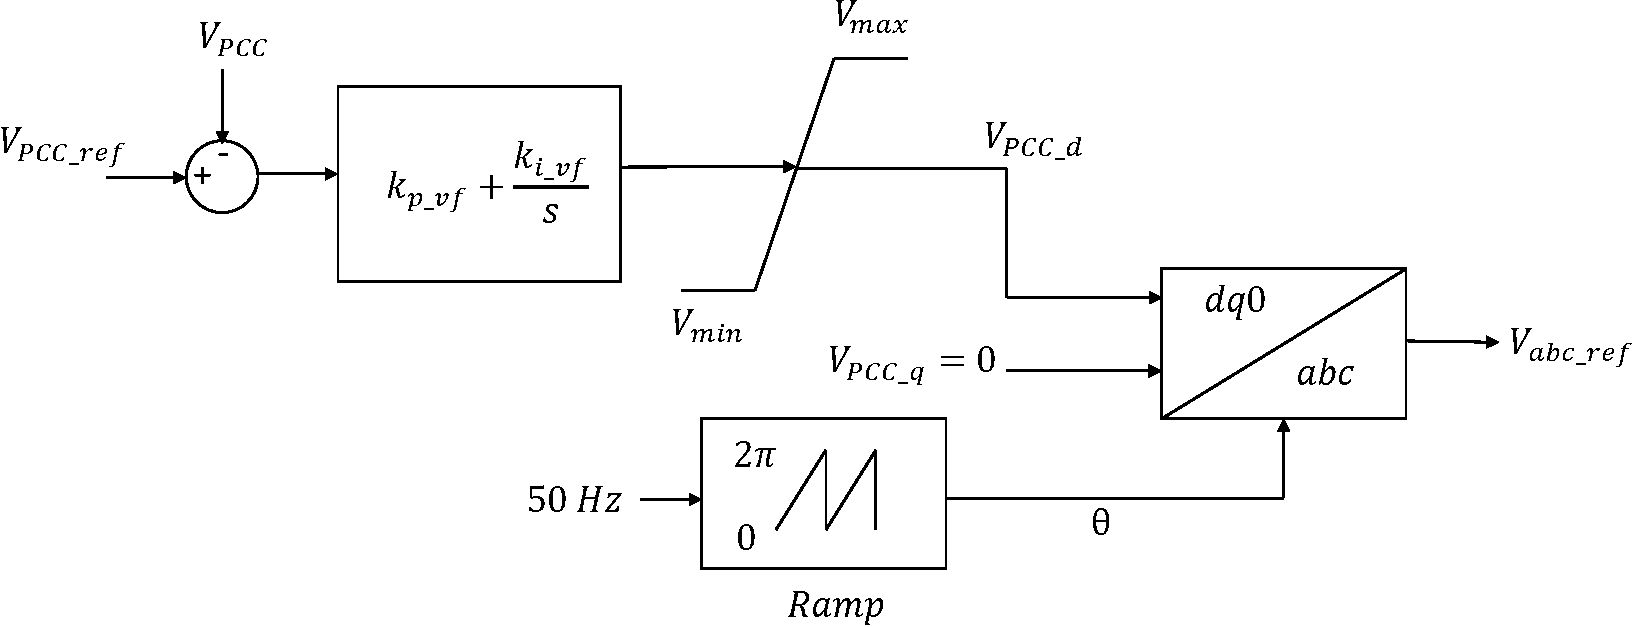
\includegraphics[height = 5cm,width = 12.5cm]{Diagrams/Chapter_4/U_F_control.pdf}
    \caption{V/F control in MMC-1 \cite{vrana2013cigre}}
    \label{fig:U_F_control}
\end{figure}


\subsection{Non- island mode control}
This mode of operation is based on the conventional current control (grid following) approach, which consists of the outer control loop and the inner control loop. The outer loop consists of the d and q axes loops. The d-axis loop can provide control of \gls{DC} voltage or active power and the q-axis loop can provide control of \gls{AC} voltage or reactive power as depicted in Figure \ref{Control_loop_MMC_Id} and Figure \ref{Control_loop_MMC_Iq} respectively. The outer control loop provides the respective current reference values as inputs for the inner current loops. \gls{MMC}-2 is configured with this control in this work. 

The parameters defined in this section are mathematically derived as given in \cite{saad2015modelisation}. The rotating dq frame provides a simplified control of the three-phase systems. As described in Section \ref{ref_frame_trafo} and mentioned in Figure \ref{fig:DQTransformation}, the currents and voltages in the abc frame are transformed into \gls{dq} frame using Clarke-Park transformation.
As conventionally followed, the d-axis voltage is aligned with the grid voltage at the \gls{HV} bus of IT-2a interface transformer ($V_{PCC\_d\_2}$) and the q-axis is set to zero. This provides constant values for d and q components during steady state.

If active power is the priority in d-axis, active power control of \gls{MMC}-2 is given by Equations \ref{activ_pow_MMC2_eq_1} and \ref{activ_pow_MMC2_eq_2}.

\begin{equation}\label{activ_pow_MMC2_eq_1}
    P_{AC\_2} = V_{PCC\_d\_2} \times i_{d\_2}
\end{equation}

\begin{equation}\label{activ_pow_MMC2_eq_2}
    i_{d\_ref\_2} =  \frac{1}{V_{PCC\_d\_2}} \left(\frac{k_{i_P}}{s}\right)\left(P_{AC\_ref\_2}-P_{AC\_2}\right)
\end{equation}

If \gls{DC} voltage is the priority in d-axis, \gls{DC} voltage control is provided by the following equation:

\begin{equation}
    i_{d\_ref\_2} = C_{V_{DC\_2}}\left(s\right) \times \left(V_{DC\_ref\_2} - V_{DC\_2}\right)
\end{equation}

where $C_{V_{DC\_2}}$ is the transfer function of the \gls{DC} voltage control.

If reactive power is the priority in q-axis, reactive power control of \gls{MMC}-2 is given by the following equations:

\begin{equation}\label{reactiv_pow_MMC2_eq_1}
    Q_{AC\_2} = -V_{PCC\_d\_2} \times i_{q\_2}
\end{equation}

\begin{equation}\label{reactiv_pow_MMC2_eq_2}
    i_{q\_ref\_2} = -  \frac{1}{V_{PCC\_d\_2}} \left(\frac{k_{i_Q}}{s}\right)\left(Q_{AC\_ref\_2}-Q_{AC\_2}\right)
\end{equation}

The voltage difference at the equivalent reactance interface is calculated as following:

\begin{equation}\label{ac_vol_MMC2_eq_2}
    \Delta V_{PCC\_2} = V_{conv\_2} - V_{PCC\_2} \approx \frac{\omega(L_{trafo\_2}+L_{arm\_2}/2)Q_{AC\_2}}{V_{PCC\_2}}
\end{equation}

where $L_{trafo\_2}$ is the interface transformer (IT-2b) leakage reactance and $L_{arm\_2}$ is the arm inductance in \gls{MMC}-2.

Since the d-axis voltage is aligned with the grid voltage, inserting Equation \ref{reactiv_pow_MMC2_eq_1} in Equation \ref{ac_vol_MMC2_eq_2}, the following equation is obtained:

\begin{equation}
   \Delta V_{PCC\_2} \approx \omega(L_{trafo\_2}+L_{arm\_2}/2)\times i_{q\_2}
\end{equation}

The control of \gls{AC} voltage is obtained with the following equation:

\begin{equation}
    i_{q\_ref\_2} =  \left(\frac{k_{i_V}}{s}\right)\left(V_{PCC\_{ref}\_2}-V_{PCC\_2}\right)
\end{equation}

The inner loop consists of \gls{PI} controllers for d and q axis separately and provides a decoupled control action. The output from the inner loop control is then translated back to the abc frame using \gls{dq} to abc frame transformation. 

\begin{figure}[H]
\centering

%\hspace{4cm}
\subfloat[Outer control loop representation for d-axis ($i_{d\_ref\_2}$)]{%
  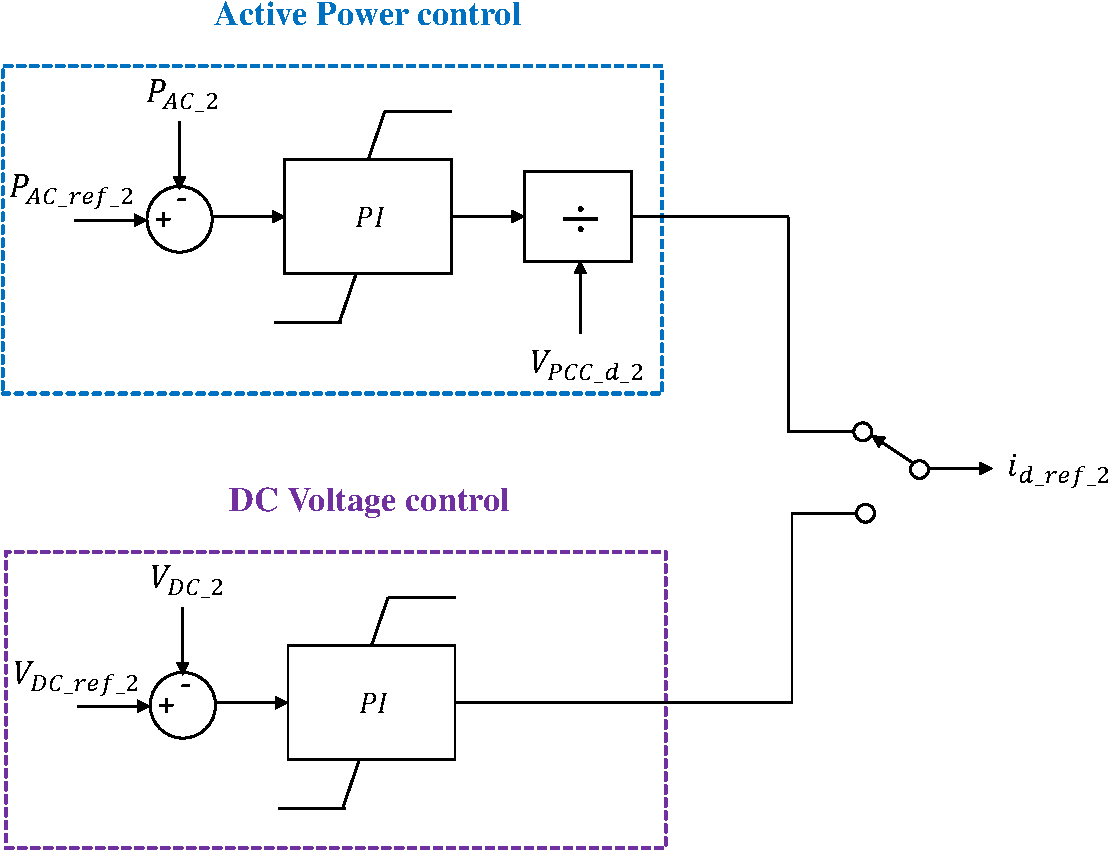
\includegraphics[clip,width=0.65\columnwidth]{Diagrams/Chapter_4/Control_loop_MMC_Id.pdf}%
\label{Control_loop_MMC_Id}}

\vspace{10mm}
%\hspace{4cm}
\subfloat[Outer control loop representation for q-axis ($i_{q\_ref\_2}$)]{%
  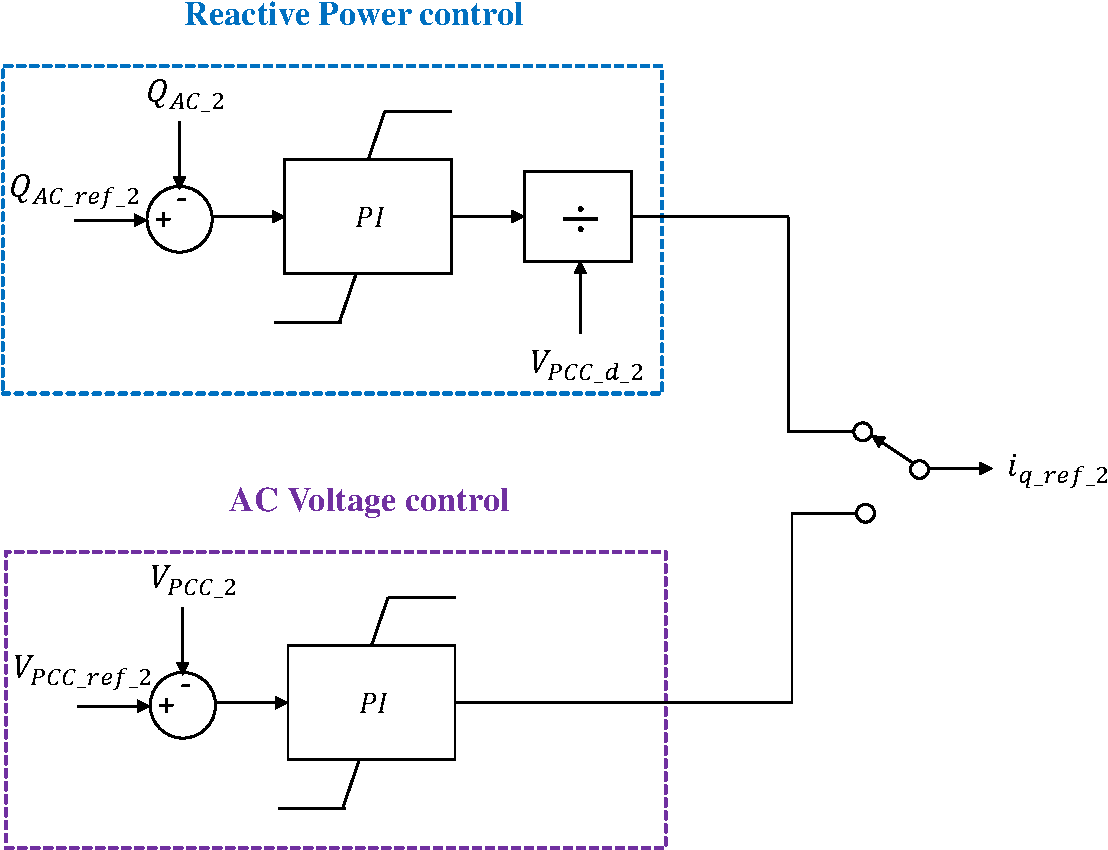
\includegraphics[clip,width=0.65\columnwidth]{Diagrams/Chapter_4/Control_loop_MMC_Iq.pdf}%
\label{Control_loop_MMC_Iq}}


\caption{Simplified structure of the outer loop control for MMC-2 \cite{saad2015modelisation}}

\end{figure}

As the \gls{DC} voltage in the \gls{HVDC} link is maintained and controlled by the onshore equivalent \gls{MMC} station represented by a constant \gls{DC} source, the active power control is chosen as priority for d-axis for \gls{MMC}-2 control. Similarly, as the \gls{AC} voltage is controlled by the V/F control in \gls{MMC}-1, reactive power control is chosen as priority chosen for q-axis for \gls{MMC}-2. When active power is the chosen priority, $P_{AC\_2}$ represents the required amount of active power that flows through offshore converter station-2 and must be defined externally by the user. However, the outer loop control available for non-islanded mode in \cite{vrana2013cigre} is not suitable for parallel operation with V/F control. Hence, the outer loop is simplified and the reference points ($i_{d\_ref\_2}$ and $i_{q\_ref\_2}$) for the inner loop are controlled directly by the user. This modification in outer loop and the power flow control in \gls{MMC}-2 in RSCAD is detailed in Appendix \ref{modific_outer_loop}.  


The inner control loop consists of \gls{PI} controllers that play the major role in ensuring minimum steady state error. The inner control also contain the feed-forward term to compensate the cross coupling terms. The mathematical equations for the parameters of inner control loop are derived as provided in \cite{saad2015modelisation}. Applying Kirchoff's Voltage Law in Figure \ref{fig:MMC_pow_system_1} and with the \gls{MMC} representation in Figure \ref{fig:MMC_pow_system_2}, the equations are derived for offshore converter station-2 connected to the \gls{AC} network. The assumptions involve, the direction of current is from the \gls{AC} network to the \gls{MMC} (similar to the condition when offshore wind power is transferred from the offshore network to onshore system) and avoiding the star-point reactor:

\begin{equation}
    \frac{V_{DC\_2}}{2} = v_{uj} + L_{arm\_2}\frac{di_{uj}}{dt} + R_{arm\_2}i_{uj} - L_{trafo\_2}\frac{di_{j}}{dt} - R_{trafo\_2}i_j + v_{PCC_j}
\end{equation}

\begin{equation}
    \frac{V_{DC\_2}}{2} = v_{lj} + L_{arm\_2}\frac{di_{lj}}{dt} + R_{arm\_2}i_{lj} + L_{trafo\_2}\frac{di_{j}}{dt} + R_{trafo\_2}i_j - v_{PCC_j}
\end{equation}

where $R_{trafo\_2}$ is the interface transformer (IT-2b) resistance, $R_{arm\_2}$ is the arm resistance in \gls{MMC}-2, $j$ represents phases $a$, $b$ and $c$. $u$ and $l$ denotes the upper arm and lower arm of \gls{MMC}-2 respectively.

\begin{figure}[H]
\centering
%\hspace*{-1.2cm}
    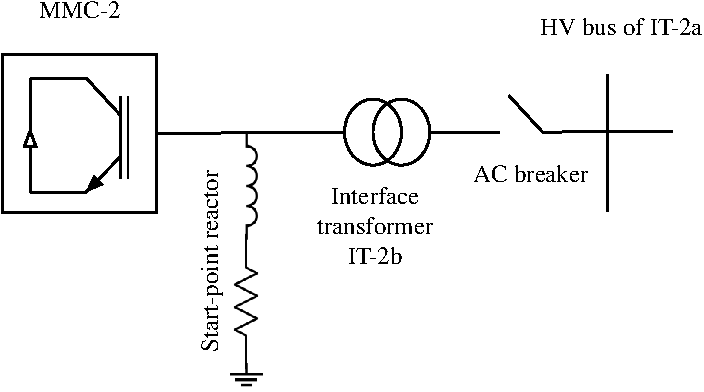
\includegraphics[height = 5cm,width = 9cm]{Diagrams/Chapter_4/MMC_pow_system_1_new.pdf}
    \caption{Representation of offshore MMC-2 station connection to the AC network \cite{saad2015modelisation}}
    \label{fig:MMC_pow_system_1}
\end{figure}

\begin{figure}[H]
\centering
%\hspace*{-1.2cm}
    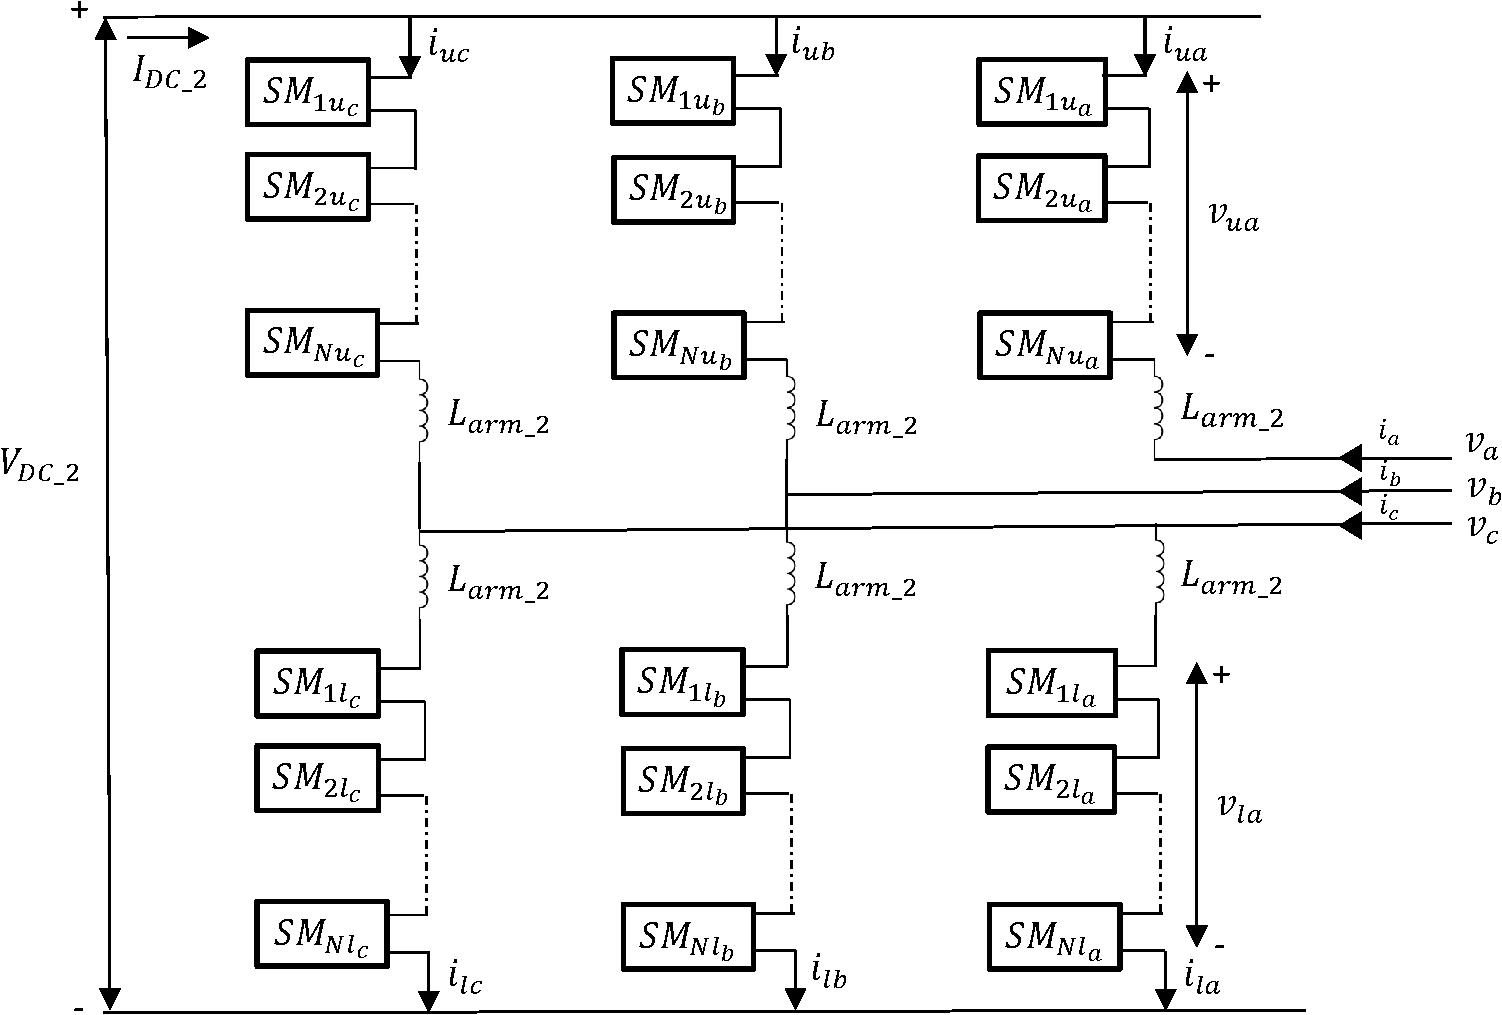
\includegraphics[height = 9cm,width = 13.5cm]{Diagrams/Chapter_4/MMC_pow_system_2.pdf}
    \caption{MMC-2 representation \cite{saad2015modelisation}}
    \label{fig:MMC_pow_system_2}
\end{figure}

The equations in \gls{dq} frame can be represented as following:

\begin{equation}
    V_{PCC\_d\_2} - V_{conv\_d\_2} = \left(\frac{L_{arm\_2}}{2} + L_{trafo\_2}\right)\frac{di_{d}}{dt} +\left (\frac{R_{arm\_2}}{2}+R_{trafo\_2}\right)i_d-\omega\left(\frac{L_{arm\_2}}{2}+L_{trafo\_2}\right)i_q
\end{equation}

\begin{equation}
    V_{PCC\_q\_2} - V_{conv\_q\_2} = \left(\frac{L_{arm\_2}}{2} + L_{trafo\_2}\right)\frac{di_{q}}{dt} +\left (\frac{R_{arm\_2}}{2}+R_{trafo\_2}\right)i_q+\omega\left(\frac{L_{arm\_2}}{2}+L_{trafo\_2}\right)i_d
\end{equation}

The control loop is defined as follows:

\begin{equation}
    V_{conv\_ref\_d\_2} = - \left(i_{d\_ref\_2} - i_d\right)C_{i_{ac}}\left(s\right) + V_{PCC\_d\_2} + \omega\left(\frac{L_{arm\_2}}{2}+L_{trafo\_2}\right)i_q
\end{equation}

\begin{equation}
    V_{conv\_ref\_q\_2} = - \left(i_{q\_ref\_2} - i_q\right)C_{i_{ac}}\left(s\right) + V_{PCC\_q\_2} + \omega\left(\frac{L_{arm\_2}}{2}-L_{trafo\_2}\right)i_d
\end{equation}

where $C_{i_{ac}}\left(s\right)$ is the transfer function of the \gls{PI} controller.

The inner control loop provides the control of reference voltages, as depicted in Figure \ref{fig:Inner_control_loop_MMC}, which are then used as inputs for the lower level control.

\begin{figure}[H]
\centering
%\hspace*{-1.2cm}
    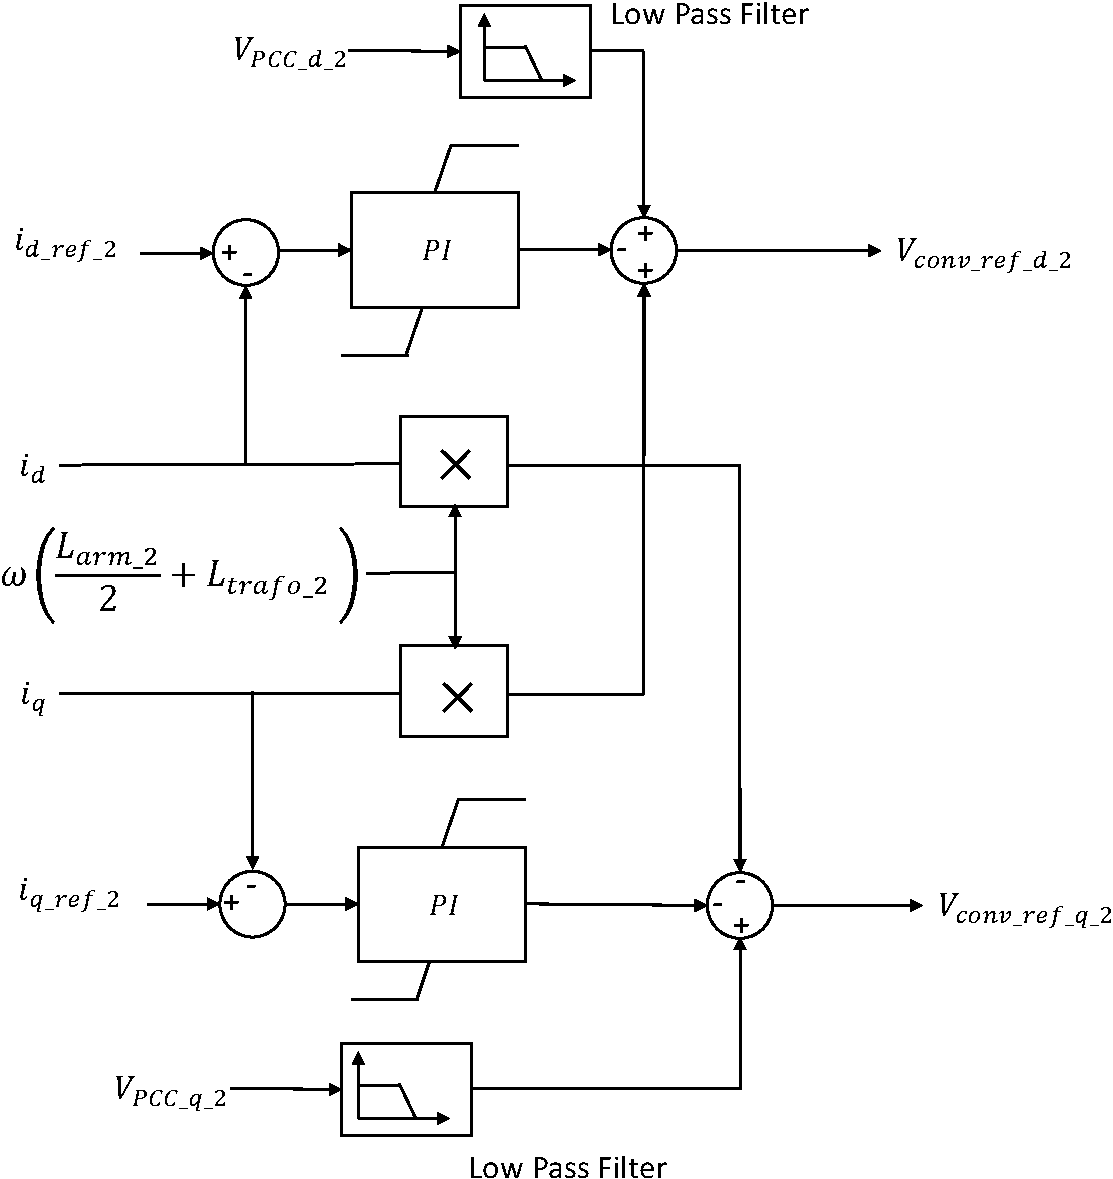
\includegraphics[height = 12cm,width = 10.5cm]{Diagrams/Chapter_4/Inner_control_loop_MMC.pdf}
    \caption{Inner loop control for MMC-2 \cite{saad2015modelisation}}
    \label{fig:Inner_control_loop_MMC}
\end{figure}

The inner control loop model available in \cite{vrana2013cigre} is only suitable for a 145 kV \gls{HVAC} network. This is why a second interface transformer (IT-2a) is used to convert the 66 kV \gls{HVAC} voltage to 145 kV, as shown in Figure \ref{fig:WT4_MMC2}. To mitigate the effect of this transformer in terms of impedance, the leakage reactance and resistance of the transformer are kept to a minimum value (0.001 p.u.). However, it should be noted that, this is a work around approach used in this work and such a transformer with very low reactance is not practically used in a power system network. The non-island mode control in \gls{MMC}-2 identifies the frequency and phase angle at the \gls{HV} bus of the interface transformer (IT-2a) in Figure \ref{fig:WT4_MMC2}. The \gls{PLL} in \gls{MMC}-2 control, performs this task and synchronizes with the measured grid voltage at the \gls{HV} bus of IT-2a. The \gls{PI} gains for the \gls{PLL} were set based on parameter sensitivity analysis. The phase angle is generated by the \gls{PLL} which is used to transform it from abc to \gls{dq} frame.

The lower level controls such as circulating current suppression control, modulation and third harmonic injection %and current limiter 
are available in the average \gls{EMT} model of \gls{MMC} controls in \cite{vrana2013cigre} and are used as such for this work in both \gls{MMC}-1 and \gls{MMC}-2. Further, the performance of the 2 GW offshore network is to be analyzed during steady state and dynamic conditions after incorporating the aforementioned control strategies.

